% !TEX root = _individual/flatland.tex

%%%%%%%%%%%%%%%%%%%%%%%%%%%%%%%%%%%%%%%%%%%%%%%%%%%%%%%%%%%%%%%%%%%%%%%%%%%%%%%%
\chapter{Flatland Geometry}

Flatland geometry is a fictional two-dimensional space where particles are
constrained to the page \cite{Abb1884,Asa2008}. This differs from standard 2-D
geometry, which represents a 3-D problem that is invariant in the $z$ axis,
where particles can travel at different polar angles out of the page. The
constraint of living in the page reduces the phase space of the transport
equation, as the flatland solution is only a function of the azimuthal angle
rather than both azimuthal and polar angles. This reduction in phase space makes 
flatland geometry a computationally less burdensome testing ground for new
methods.

Despite being easier computationally to solve, flatland has a few subtle quirks
that need to be taken into account before implementing a solver in that
geometry. Previous work in flatland \cite{Asa2008,Lar2009c} has shown that the
diffusion coefficient for flatland geometry $\frac{1}{2\sigma}$ is different from
the physical diffusion coefficients $\frac{1}{3\sigma}$, but the correct
formulation for flatland diffusion boundary
conditions have remained an unanswered and indeed unasked question. This
chapter answers that question in addition to providing other insights into this
strange geometry.

%%%%%%%%%%%%%%%%%%%%%%%%%%%%%%%%%%%%%%%%%%%%%%%%%%%%%%%%%%%%%%%%%%%%%%%%%%%%%%%%
\section{Transport in flatland}

Two-dimensional $x$-$y$ geometry represents a three-dimensional problem that is
invariant in the $z$ direction. 

\begin{sidewaystable}[hp]
  \centering
  \renewcommand*{\arraystretch}{1.5}
  \begin{tabular}{rcccccc}
\toprule
   Geometry & $\vec{\Omega}$ & Domain $\Omega$ & $\ud\Omega$
   & $\omega_0 \equiv \int_\Omega \ud\Omega$
   & $\omega_1 \equiv \int_\Omega \abs{\vec{\Omega}\vd\vec{i}} \ud\Omega$
   & $\omega_2 \equiv \int_\Omega (\vec{\Omega}\vd\vec{i})^2 \ud\Omega$
\\ \midrule
   1D & $\mu$ & $-1 \le \mu \le 1$ & $\ud\mu$
   & 2 & 1 & $\frac{2}{3}$
   \\
   2D & $\sqrt{1-\mu^2} \cos \theta \vec{i}
   + \sqrt{1-\mu^2} \sin \theta \vec{j}$
   & $-1 \le \mu \le 1$, $0 \le \theta < 2\pi$ & $\ud\mu \ud \theta$
   & $4\pi$ & $2\pi$ & $\frac{4\pi}{3}$
   \\
   Flatland & $\cos \theta \vec{i} + \sin \theta \vec{j}$
   & $0 \le \theta < 2\pi$ & $\ud \theta$
   & $2\pi$ & $4$ & $\pi$
   \\
   3D & $\mu \vec{i}
   + \sqrt{1-\mu^2} \cos \theta \vec{j}
   + \sqrt{1-\mu^2} \sin \theta \vec{k}$
   & $-1 \le \mu \le 1$, $0 \le \theta < 2\pi$ & $\ud\mu \ud \theta$
   & $4\pi$ & $2\pi$ & $\frac{4\pi}{3}$
\\ \bottomrule
  \end{tabular}
  \caption{Geometry descriptions and identities.}
  \label{tab:geometry}
\end{sidewaystable}

%%%%%%%%%%%%%%%%%%%%%%%%%%%%%%%%%%%%%%%%
\clearpage
\subsection{An insightful comparison problem}

On paper, the problem looks like Fig.~\ref{fig:chordFlatland}, where $\theta$
is the azimuthal angle in both flatland and 2-D geometry. However, in flatland,
the line of length $s$ is constrained to the plane, where in 2D, $s$ is the
length of the distance projected onto the plane. The line actually 
\begin{figure}[htb]
  \centering
  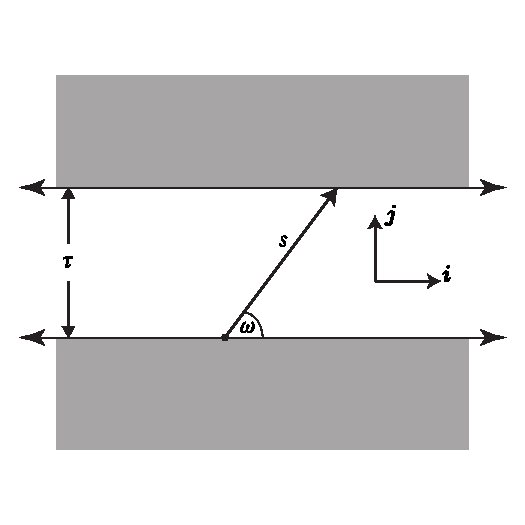
\includegraphics{chord-flatland}
  \caption[The chord length problem as represented on paper.]%
  {The chord length problem as represented on paper. The gap is
  $\tau$ mean free paths apart, $\theta$ is the azimuthal angle, and $s$ is the
  distance across the gap.}
  \label{fig:chordFlatland}
\end{figure}

\begin{figure}[htb]
  \centering
  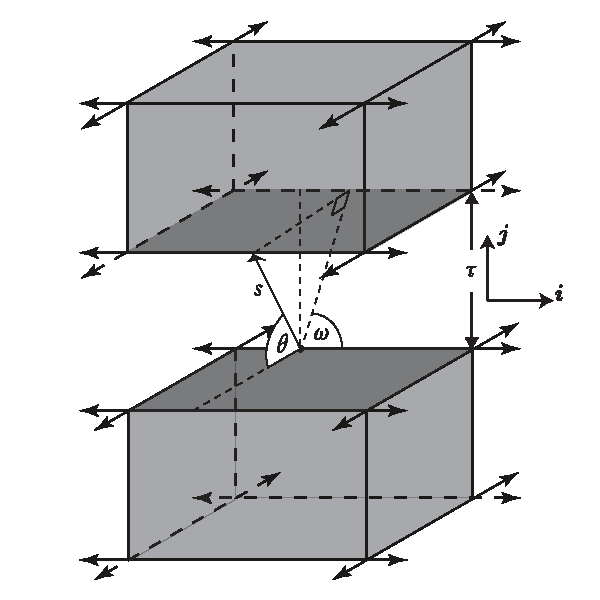
\includegraphics{chord-xyz}
  \caption[A more full view of the chord length problem in 2-D geometry.]%
  {A more full view of the chord length problem in 2-D geometry.
  The polar angle cosine is $\mu= \cos \varphi$, and the azimuthal angle is
  $\theta$.}
  \label{fig:chordFlatland}
\end{figure}

\begin{figure}[htb]
  \centering
  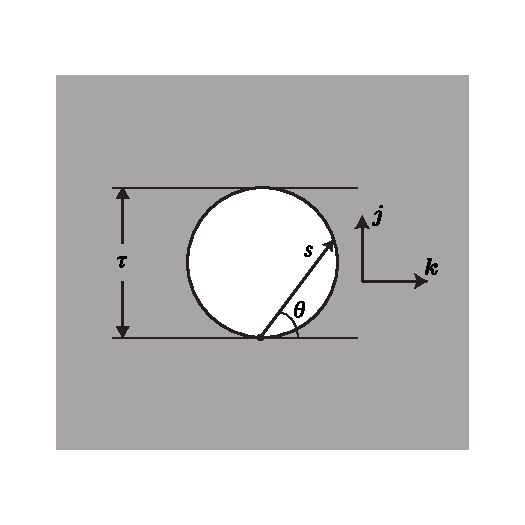
\includegraphics{chord-rz}
  \caption[A cross-section of the chord length problem in $r$--$z$
  geometry.]%
  {A cross-section of the chord length problem in $r$--$z$
  geometry. The orthogonal view looks like Fig.~\ref{fig:chordFlatland}.}
  \label{fig:chordRz}
\end{figure}

Flatland probability of reaching other side:
\begin{equation*}
  p(\tau) = \frac{\int_{0}^{\pi} \eexp^{-\tau / \sin \theta} \sin \theta \ud
  \theta}{\int_{0}^{\pi} \sin \theta \ud \theta}
  = \frac{1}{2} \int_{0}^{\pi} \eexp^{-\tau / \sin \theta} \sin \theta \ud
  \theta
\end{equation*}

2-D probability of reaching other side:
\begin{equation*}
  p(\tau) = \frac{\int_{0}^{\pi} \int_{-1}^{1} \eexp^{-\tau / \left(
  \sqrt{1-\mu^2} \sin\theta \right)}
  \sqrt{1-\mu^2} \sin\theta \ud\mu \ud \theta}
  {\int_{0}^{\pi} \int_{-1}^{1} \sqrt{1-\mu^2} \sin\theta \ud\mu \ud\theta}
  = \frac{\int_{0}^{2\pi} \int_{0}^{1} \eexp^{-\tau / \mu} \mu
  \ud\mu \ud\theta }
  {\int_{0}^{2\pi} \int_{0}^{1} \mu \ud\mu \ud\theta}
  = 2 \int_{0}^{1} \eexp^{-\tau / \mu} \mu
  \ud\mu
\end{equation*}

Cylindrical probability of reaching other side:
\begin{equation*}
  p(\tau) = \frac{\int_{0}^{\pi} \int_{-1}^{1} \eexp^{-\tau \sin \theta / 
  \sqrt{1-\mu^2}}
  \sqrt{1-\mu^2} \sin\theta \ud\mu \ud \theta}
  {\int_{0}^{\pi} \int_{-1}^{1} \sqrt{1-\mu^2} \sin\theta \ud\mu \ud\theta}
  = \frac{1}{\pi} \int_{0}^{\pi} \int_{-1}^{1} \eexp^{-\tau \sin \theta / 
  \sqrt{1-\mu^2}}
  \sqrt{1-\mu^2} \sin\theta \ud\mu \ud \theta
\end{equation*}

\begin{table}[htb]
  \centering
  \begin{tabular}{llll}
\toprule
\phantom{10}$\tau$ & $r$--$z$ & Flatland & $x$--$y$
\\ \midrule
           0.01 & 0.990 & 0.985 & 0.981 \\
\phantom{1}0.1 & 0.906 & 0.863 & 0.833 \\
\phantom{1}1 & 0.404 & 0.274 & 0.219 \\
\phantom{1}10 & 0.00772 & 1.63\EE{-5} & 7.10\EE{-6}
 \\
\bottomrule
  \end{tabular}
  \caption{Comparison of the probability of crossing a channel $\tau$ mfp thick
  without colliding.}
  \label{tab:collision}
\end{table}

%%%%%%%%%%%%%%%%%%%%%%%%%%%%%%%%%%%%%%%%
\clearpage
\subsection{Monte Carlo sampling}
\cite{Lew1984,Bro2004a}
Direct sampling 
probability distribution function (PDF)
cumulative distribution function (CDF)

\subsubsection{Isotropic volume source}
An isotropic internal source, whether directly from an extraneous radiation
source or indirectly from isotropic scattering, has an equal probability of
entering any angle. The normalized  that
represents this process is
\begin{equation*}
  f(\theta) \ud \theta = \frac{1}{2\pi} \ud \theta\,, \quad \theta \in [0, 2\pi)\,.
\end{equation*}
To sample the angle that results from an isotropic event, we use the :
\begin{equation*}
  F(\theta) = \int_{0}^{\theta} f(\theta') \ud \theta' = \frac{1}{2\pi}
  \theta\,.
\end{equation*}
Setting $\xi_1 = F(\theta)$ and solving for $\theta = F\inv(\xi_1)$ gives the
simple result that
\begin{equation*}
  \theta = 2\pi \xi_1\,.
\end{equation*}
The particle's new angle is therefore
\begin{equation*}
  \vec{\Omega} = \cos \theta \vec{i} + \sin \theta \vec{j}
  = \cos 2\pi\xi_1\vec{i} + \sin 2\pi\xi_1 \vec{j}\,.
\end{equation*}

\subsubsection{Isotropic surface source}
Particles emitted from an isotropic surface source have a cosine distribution
\cite{Gre2002}, which makes constant the radiation flux in each differential
angle:
\begin{equation}\label{eq:surfaceSource}
  f(\vec{\Omega}) \ud \Omega = c \abs{\vec{\Omega}\vd \vec{n}} \ud \Omega \,,
\vec{\Omega}\vd \vec{n} < 0 \,,
\end{equation}
where $c$ is a normalization constant.

In 3D, with $\vec{n}=\vec{i}$ so $\abs{\vec{\Omega}\vd \vec{n}}=\mu$, this has
the form
\begin{equation*}
  f(\mu, \theta) \ud\mu \ud\theta = \frac{\mu \ud\mu}{2} \frac{\ud\theta}{2\pi}
  \,,\quad 0 \le \mu < 1\,,\ 0 \le \theta < 2\pi\,,
\end{equation*}
a separable distribution that gives $\mu=\sqrt{\xi_1}$ and $\theta=2\pi \xi_2$.

For flatland geometry, the representation is different. Let us choose
$\vec{n} = -\vec{j}$ so that incident directions are inside
$\theta \in [0, \pi)$.
Applying the flatland identities in Table~\ref{tab:geometry} to
Eq.~\eqref{eq:surfaceSource} gives
\begin{equation*}
  f(\theta) \ud\theta = c\abs{ -\sin \theta}
  = c \sin \theta \,,\quad 0 \le \theta < \pi\,.
\end{equation*}
Integrating this gives
\begin{equation*}
  F(\theta) \ud\theta = c \left( 1-\cos\theta \right)
  \,,\quad 0 \le \theta < \pi\,,
\end{equation*}
The constant $c$ should satisfy $F(\pi)=1$:
\begin{equation*}
  1 = c (1 - (-1) ) \lra c=\frac{1}{2}\,.
\end{equation*}

Thus, the CDF for particle emission from a surface source in flatland geometry
is
\begin{equation*}
  F(\theta) \ud\theta = \frac{1}{2} \left( 1-\cos\theta \right)
  \,,\quad 0 \le \theta < \pi\,.
\end{equation*}
Solving for $\theta = F\inv(\xi_1)$ gives a sampled angle for a surface source
in flatland:
\begin{equation*}
  \theta = \cos\inv(1 - 2\xi_1)\,.
\end{equation*}
Using the identity $\cos^2 \theta + \sin^2 \theta = 1$, the particle's new angle is
\begin{align*}
  \vec{\Omega} &= \cos \theta \vec{i} + \sin \theta \vec{j} \\
  &=  \cos[ \cos\inv(1 - 2\xi_1) ] \vec{i} + \sin[ \cos\inv(1 - 2\xi_1) ] \vec{j} \\
  &= (1 - 2\xi_1) \vec{i} + \sqrt{1 - (1 - 2\xi_1)^2} \vec{j}\,.
\end{align*}

%%%%%%%%%%%%%%%%%%%%%%%%%%%%%%%%%%%%%%%%%%%%%%%%%%%%%%%%%%%%%%%%%%%%%%%%%%%%%%%%
\section{Diffusion in flatland}

%%%%%%%%%%%%%%%%%%%%%%%%%%%%%%%%%%%%%%%%
\subsection{Interior diffusion approximation}

%%%%%%%%%%%%%%%%%%%%%%%%%%%%%%%%%%%%%%%%
\subsection{Boundary conditions}

``Marshak'' extrapolation distance:
\begin{equation*}
  z = \frac{\pi}{4} \approx 0.78540
\end{equation*}
Variational extrapolation distance:
\begin{equation*}
  z = \frac{\pi}{8} + \frac{4}{3\pi} \approx 0.81711
\end{equation*}

%%%%%%%%%%%%%%%%%%%%%%%%%%%%%%%%%%%%%%%%%%%%%%%%%%%%%%%%%%%%%%%%%%%%%%%%%%%%%%%%

